%
% Showcase file to demonstrate the abilities of kLabCourse-template.
% 
% 

\documentclass[ngerman]{kLCReprt}

\usepackage{blindtext}
\usepackage{kLCTitle}
\reportAuthor[Zweiter Autor]{Erster Autor}
\reportAuthorMail[zweite.mail@mail.org]{email@mail.org}
\reportDate{25.02.2015}
\reportSubmissionDate{06.03.2015}
\reportExperiment{Nummer 14}
\reportTitle{Titel des Experiments}
\reportSupervisor{Mein Supervisor}

\bibliography{bib/bibliography.bib}


\begin{document}
\maketitle\thispagestyle{empty}
\cleardoublepage
\tableofcontents\thispagestyle{plain}
\cleardoublepage

% Section with some text and heading and list levels


% \let\chapter\section
% \let\section\subsection
% \let\subsection\subsubsection

\makeatletter
% \chapter{\blindtext@heading 0 (Chapter)}
% \Blindtext
\section{\blindtext@heading 1 (section)}
\Blindtext
\subsection{\blindtext@heading 2 (subsection)}
\Blindtext
\subsubsection{\blindtext@heading 3 (subsubsection)}
\Blindtext
\paragraph{\blindtext@heading 4 (paragraph)}
\Blindtext
\section{\blindtext@list}%
\subsection{\blindtext@listEx (itemize)}%
\Blinditemize[3]
\subsection{\blindtext@listEx (4*itemize)}%
% \blind@longtrue
\blindlistlist{itemize}[2]%
\subsection{\blindtext@listEx (enumerate)}%
\Blindenumerate[3]
\subsection{\blindtext@listEx (4*enumerate)}%
% \blind@longtrue
\blindlistlist{enumerate}[2]%
\makeatother



%%% Local Variables:
%%% mode: latex
%%% TeX-master: "../diss"
%%% End:

% Section with some maths

\section{Ein Abschnitt mit Matheformeln}
\blindmathpaper


\subsection{Formeln inkl. Subequations and Labels}
\label{sec:maths-incl-subeq}
\blindtext
\newcommand{\iu}{{i\mkern1mu}}
\vspace{-.4cm}
\begin{subequations}
  \begin{align}
    \iu \hbar \partial_t \Psi &= - \iu \hbar c \sum_{i=1}^3 \alpha_i \partial_i \Psi + \beta m c^2 \Psi\\ &= \left( c \vec \alpha \cdot \vec p + \beta m c^2 \right) \Psi \\
    \Longrightarrow \quad 0 &= \left( \iu \hbar \gamma^\mu \partial_\mu - mc \right) \Psi
  \end{align}
\end{subequations}
\blindtext
\begin{align}
  F(x,y)=0 ~~\mbox{and}~~
  \left| \begin{array}{ccc}
           F''_{xx} & F''_{xy} &  F'_x \\
           F''_{yx} & F''_{yy} &  F'_y \\
           F'_x     & F'_y     & 0
         \end{array}\right| = 0
\label{eq:1}
\end{align}
\blindtext


% End of file

% Section with miscellaneous contents


\section{Sonstiges (Floats, Zitationen, etc.)}


\subsection{Unterabschnitt mit Zitationen}
Dies ist eine Zitation~\cite{D0.ConfNote.5607} und dies eine weitere~\cite{PhysRevLett.100.192004}. Und mehrere Zitationen auf einmal~\cite{PhysRevLett.74.2632, PhysRevLett.100.192004, PhysRevLett.74.2626}.
\blindtext


\subsection{Unterabschnitt mit Figures}
\blindtext
%
\begin{figure*}[t]
  \centering
  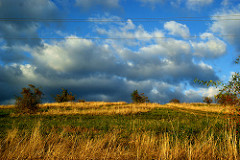
\includegraphics[width=0.49\textwidth]{example.jpg}
  \caption{\blindtext}
  \label{fig:1}
\end{figure*}
%
\blindtext
%
\begin{figure}[t]
  \centering
  \subcaptionbox{\label{fig:3.1}Erste Bildunterschrift.}{%
    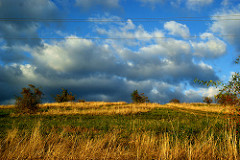
\includegraphics[width=0.24\textwidth]{example.jpg}%
  }~
  \subcaptionbox{\label{fig:3.2}Zweite Bildunterschrift.}{%
    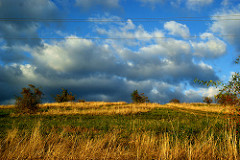
\includegraphics[width=0.24\textwidth]{example.jpg}
  }
  \caption{Bildunterschrift der gesamten Figure mit Referenzen auf~\cref{fig:3.1} and~\cref{fig:3.2}.}
  \label{fig:3}
\end{figure}
%
\blindtext


\subsection{Unterabschnitt mit Referenzen}
Dies hier ist eine Referenz auf \cref{fig:1}. Und dies eine andere Referenz auf \cref{eq:1}, welche sich in \cref{sec:maths-incl-subeq} befindet. Und das hier ist eine Referenz auf \cref{fig:3.1}, welche Teil von \cref{fig:3} ist. \blindtext


\subsection{Unterabschnitt mit Tabelle}
\blindtext

\begin{table}[tb]
  \centering
  \caption{Dies ist die Tabellenbeschreibung.}
  \begin{tabular}{l l l l l l l}
    \toprule
    OrderDate & Region & Rep & Item & Units & Cost & Total \\
    \midrule
    1/6/2014 & East & Jones & Pencil & 95 & 1.99 & 189.05 \\
    1/23/2014 & Central & Kivell & Binder & 50 & 19.99 & 999.50 \\
    2/9/2014 & Central & Jardine & Pencil & 36 & 4.99 & 179.64 \\
    2/26/2014 & Central & Gill & Pen & 27 & 19.99 & 539.73 \\
    3/15/2014 & West & Sorvino & Pencil & 56 & 2.99 & 167.44 \\
    4/1/2014 & East & Jones & Binder & 60 & 4.99 & 299.40 \\
    4/18/2014 & Central & Andrews & Pencil & 75 & 1.99 & 149.25 \\
    5/5/2014 & Central & Jardine & Pencil & 90 & 4.99 & 449.10 \\
    \bottomrule
  \end{tabular}
  \label{tab:1}
\end{table}
%
\blindtext


% End of file

% Section with font examples


\newcommand*{\abc}{abcdefghijklmnopqrstuvwxyz}
\newcommand*{\ABC}{ABCDEFGHIJKLMNOPQRSTUVWXYZ}


\section{Different Font Examples}


\subsection{Subsection with Font Examples (Roman)}

\begin{quotation}
\noindent
\large
\begin{tabular}{l l}
Caps:    & \ABC \\
         & \abc \\
SC:      & \textsc{\abc} \\
Italics: & abcefghijop ~ \textit{abcefghijopy} \\
Ligatures: & Fancy \textit{flesh} fresh \textsc{Blood} final\\
OSF:     & 0123456789 ~~ $0123456789$ \\
\end{tabular}
\end{quotation}


\subsection{Subsection with Font Examples (Sansserif)}

\begin{quotation}
\noindent
\large
\sffamily
\begin{tabular}{l l}
Caps:    & \ABC \\
         & \abc \\
SC:      & \textsc{\abc} \\
Italics: & abcefghijop ~ \textit{abcefghijopy} \\
Ligatures: & Fancy \textit{flesh} fresh \textsc{Blood} final\\
OSF:     & 0123456789 ~~ $\mathsf{0123456789}$ \\
\end{tabular}
\end{quotation}


\subsection{Example of Italic Inline Text}
\renewcommand{\blindmarkup}[1]{\emph{#1}}
\blindtext


\subsection{Example of Small Caps Inline Text}
\renewcommand{\blindmarkup}[1]{\textsc{#1}}
\blindtext

\renewcommand{\blindmarkup}[1]{}


\appendix
\section{Grafiken und Tabellen}
\cleardoublepage

\printbibliography

\end{document}

% End of file
